%% Be sure to check spelling!

%% Put **your** name and the proper due date in place

\documentclass{article}
\usepackage{amsmath}    % loads AMS-Math package
\usepackage{epsfig}     % allows PostScript files
\usepackage{listings}   % allows lstlisting environment
\usepackage{moreverb}   % allows listinginput environment
\usepackage{vmargin}    % allows better margins
\setpapersize{USletter} % sets the paper size
\setmarginsrb{1in}{0.5in}{1in}{0.2in}{12pt}{11mm}{0pt}{11mm} %sets margins 
\begin{document}
\begin{center}
\rule{6.5in}{0.5mm}\\~\\
{\bf \large EGR 103L -- Fall 2016}\\~\\
{\huge \bf \LaTeX~Assignment}\\~\\
CEMAL YAGCIOGLU (cy111)\\
Lab Section 05, WEDNESDAY 11:45 AM - 2.35 PM\\
11 SEPTEMBER, 2016\\~\\ 
{\small I understand and have adhered to all the tenets of the Duke
  Community Standard in completing every part of this assignment.  I
  understand that a violation of any part of the Standard on any part
  of this assignment can result in failure of this assignment, failure
  of this course, and/or suspension from Duke University.} 
\rule{6.5in}{0.5mm}\\
\end{center}
\tableofcontents
\listoffigures
\pagebreak

\section{Equations} %%% You will add your equations here
\begin{itemize}
\item General second-order system equation\cite[p.~221]{Rizzoni}:
\begin{align*}
\frac{1}{\omega^2_n}\frac{d^2x(t)}{dt^2}+\frac{2\zeta}{\omega_n}\frac{dx(t)}{dt}+x(t)=K_\mathrm{S}f(t)
\end{align*}
\item The Secant Formula for finding maximum stress 
in a column\cite[p.~681]{Hibbeler}:
\begin{align*}
\sigma_\mathrm{max}=\frac{P}{A}\left[1+\frac{ec}{r^2}\mathrm{sec}\Bigg(\frac{L}{2r}\sqrt{\frac{P}{EA}}\Bigg)\right]
\end{align*}
\item Characteristic determinant for a 2x2 system of 
differential equations\cite[p.~152]{Kreyszig}:
\begin{align}
\nonumber \mathrm{det\left(\textbf{A}-\lambda\textbf{I}\right)} &= 
\begin{vmatrix}
a_{11}-\lambda & a_{12}  \\
a_{21} & a_{22}-\lambda
\end{vmatrix}  \\
\nonumber &=(a_{11}-\lambda)(a_{22}-\lambda)-a_{12}a_{21} \\ 
&=\lambda^2-(a_{11}+a_{22})\lambda+a_{11}a_{22}-a_{12}a_{21}=0
\end{align}
%%\end{align*}
\item Definition of the Lyapunov exponent\cite[p.~56]{Ott}:
\begin{align}
%%\abs{x}
%%\lim_{x\to\infty}x^2
h&=\lim_{T\to\infty}\frac{1}{T}\mathrm{ln}
\left|
\frac{\mathrm{d}x_T}{\mathrm{d}x_0}
\right| \\
h&=\lim_{T\to\infty}\frac{1}{T}\sum_{n=0}^{T-1}
\mathrm{ln}
\left|M'(x_n)
\right| \\
h&=\int\mathrm{ln}\left|M'(x)
\right|
d\mu(x)
\end{align}
\end{itemize}

\section{Tables using {\tt tabular} and {\tt array}}
\subsection{Using {\tt tabular}} %%% You will add the tabular here
Converting ammonia into nitric acid - the Ostwald Process\cite{Ostwald}:
\\
\begin{center}
\begin{tabular}{ r | l}
Descripton & Chemical equation \\ \hline
Oxidation of Ammonia & $4$ NH$_3$ (g) + $5$ O$_2$ $\rightarrow$ $4$ NO (g) + $6$ H$_2$O (g) \\
Oxidization of Nitric Oxide & 2 NO (g) + O$_2$ (g) $\rightarrow$ 2 NO$_2$ (g) \\
Absorption of Nitrogen Dioxide & 3 NO$_2$ (g) + H$_2$O (l) $\rightarrow$ 2 HNO$_3$ (aq) + NO (g) \\
\end{tabular}
\end{center}
\subsection{Using {\tt array}} %%% You will add the array here
\begin{center}
\renewcommand{\arraystretch}{1.5} 
\[
\begin{array}{|c|c|} \hline
\mbox{Equation} & \mbox{Description} \\
\hline
\hline
\vec{v}=v_x\hat{\imath}+v_y\hat{\jmath}+v_z\hat{k}  & \mbox{Resolution into Components} \\ \hline
v^2=v_0^2+2a\Delta x & \mbox{Velocity formula} \\ \hline
\end{array} \]
\end{center} 
\pagebreak

\section{Comments} %%% You will add your comments here
Things I learned in this assignment:
\\
\begin{itemize}
\item How to use the {\tt align} and {\tt align*} environment to typeset numbered and unnumbered equations andusing the {\tt nonumber} command to suppress numbering equations in an {\tt align} environment;
\\
\item How to use \$ to enter math mode in a line of text to type shorter mathematical expressions like  $10^6$ and $\nabla u$ or Greek letters like $\Delta$; \\

\item How to use the {\tt mathrm} command to put super- and subscripts in regular, versus italic, type for things like $V_{\mathrm{min}}$ instead of $V_{min}$;
\\
\item How to change the appearance of fonts to make words {\bf bold}, {\em italics}, or {\tt typewriter font};
\\
\item How to write mathematical formulas with commands like $\backslash$frac, $\backslash$sqrt, etc;
\\
\item How to use $\backslash$item command to write in an organized way with bullet points;
\\
\item How to use \& command before equals sign to properly arrange following equations in mathematical formulas. 
\\ 
\end{itemize}
\pagebreak
\appendix
\section{Codes}
%%% Everything in this section is done; make sure you 
%%% understand how it works in general
\subsection{Listing of full sample header for original code}
\listinginput[1]{1}{Header1f.m}

\subsection{Listing of short sample header for original code}
\listinginput[1]{1}{Header1s.m}

\subsection{Listing of full sample header for modified code}
\listinginput[1]{1}{Header2f.m}

\subsection{Listing of short sample header for modified code}
\listinginput[1]{1}{Header2s.m}

\pagebreak
\section{Figures \label{FigureList}}
%%% Almost everything in this section is done; make sure you 
%%% understand how it works in general and be sure to 
%%%uncomment the epsfig lines

\begin{figure}[htb]
\begin{center}
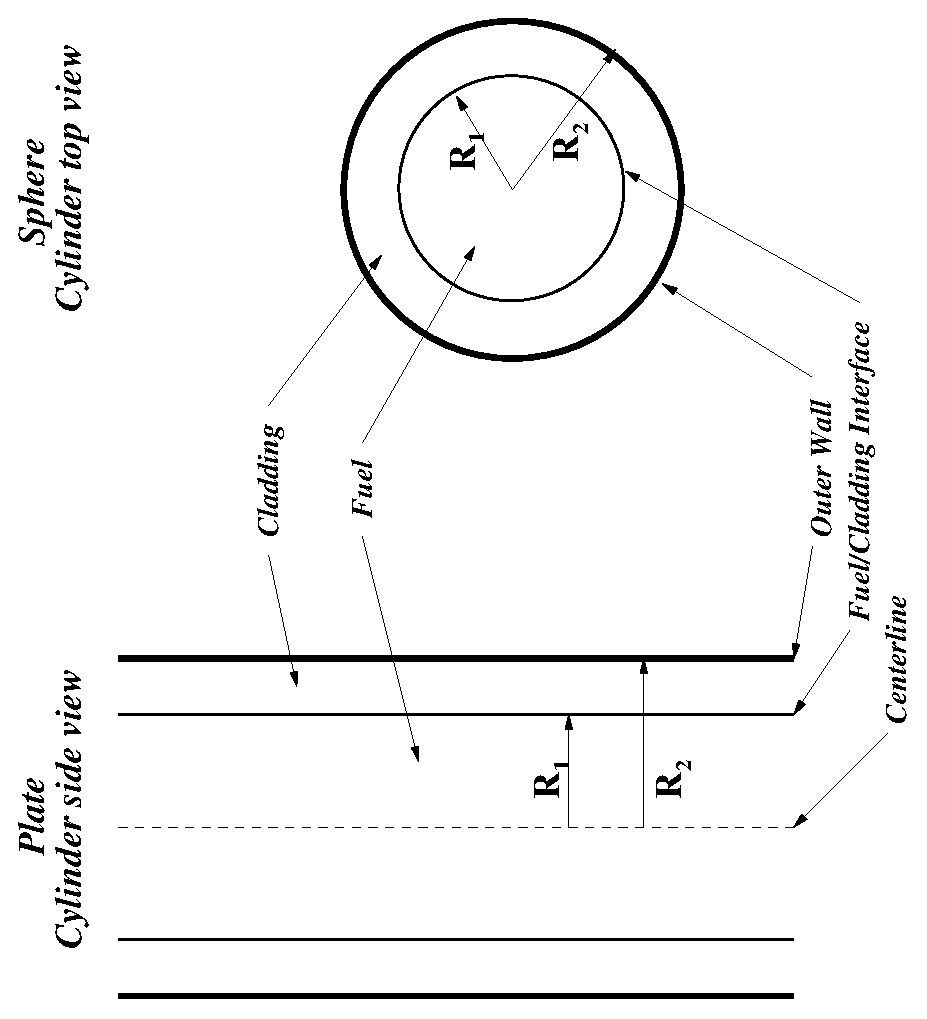
\epsfig{file=drawing.eps, width=3in, angle=-90} 
\caption{Drawing from ME 431L test.}
\end{center}
\end{figure}

\begin{figure}[htb]
\begin{center}
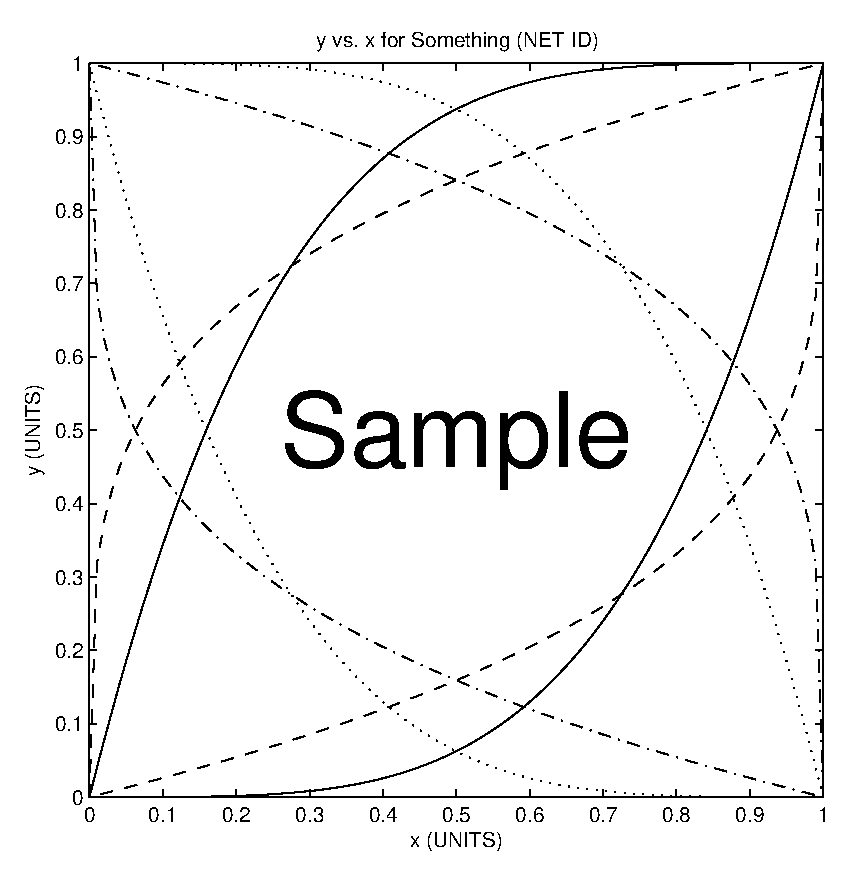
\epsfig{file=SampleFigure.eps, width=2.5in} 
\caption{Sample MATLAB figure.}
\end{center}
\end{figure}
\pagebreak

%%% Everything in this section is done; make sure you 
%%% understand how it works in general
%%% Note that line returns are optional
\addcontentsline{toc}{section}{References}
\begin{thebibliography}{9}
\bibitem{Rizzoni}
Rizzoni, Georgio,
{\it Principles and Applications of Electrical Engineering}.
McGraw-Hill, New York,
5th Edition,
2007.
\bibitem{Hibbeler}
Hibbeler, R. C.,
{\it Mechanics of Materials}.
Pearson Prentice Hall, Upper Saddle River, NJ, 8th Edition, 2011.
\bibitem{Kreyszig}
Kreyszig, Erwin,
{\it Advanced Engineering Mathematics}.
John Wiley \& Sons, New York, 8th Edition, 1999.
\bibitem{Ott}
Ott, Edward,
{\it Chaos in Dynamical Systems}.
Cambridge University Press, Cambridge, UK, 1st Edition, 1993.
\bibitem{Ostwald}
Wikipedia, 
{\it Ostwald process} (http://en.wikipedia.org/wiki/Ostwald$\_$process).
Online; accessed 19-Aug-2012.
\end{thebibliography}

\end{document}
